\chapter{Introduction and Context}

Artificial intelligence has become one of the most prominent policy issues confronting the United Kingdom's political establishment. Since the publication of the House of Lords AI Select Committee report in 2018 \parencite{hol2018} and the subsequent National AI Strategy in 2021 \parencite{hmgov2021}, successive UK governments have sought to position Britain as a global leader in AI development and governance. The trajectory of UK AI policy has been marked by a deliberate choice to avoid the comprehensive regulatory model adopted by the European Union's AI Act, instead favouring a sector-specific, ``pro-innovation'' framework that distributes regulatory responsibility across existing bodies such as the Information Commissioner's Office, the Competition and Markets Authority, and Ofcom.

This policy landscape underwent significant evolution between 2020 and 2026. The COVID-19 pandemic accelerated the deployment of algorithmic decision-making in public services, from the controversial A-level grading algorithm of 2020 to NHS diagnostic tools. The government hosted the AI Safety Summit at Bletchley Park in November 2023, establishing the AI Safety Institute as the world's first state-backed body dedicated to frontier AI evaluation \parencite{hmgov2023}. Following the 2024 general election, the incoming Labour government signalled continuity with the pro-innovation stance while introducing the AI Opportunities Action Plan in January 2025 \parencite{hmgov2025} and announcing plans for the Regulating AI for Growth Bill in 2026, which would grant existing regulators new statutory powers over AI systems. Alongside these developments, the creative industries mounted sustained opposition to AI's use of copyrighted material, and concerns over facial recognition, deepfakes, and online safety remained prominent in parliamentary discourse.

What is notable about these policy debates is the extent to which they are oriented toward the future. Because AI is an emerging technology characterised by deep uncertainty, policymakers cannot rely on conventional evidence to guide their decisions. Instead, they engage in what the sociological literature terms ``futures-making'': the construction of narratives, expectations, and imagined scenarios that justify present-day policy choices, investment priorities, and regulatory architectures \parencite{beckert2013}. These imagined futures range from utopian visions of AI-powered economic growth and public service transformation to dystopian warnings about mass unemployment, surveillance, and existential risk.

This study investigates how UK political actors imagine the future of artificial intelligence, and how these imagined futures vary across political arenas and political groups. It poses two research questions. First, what imagined futures do UK elected officials and parliamentarians communicate concerning AI? Second, how do different political groups imagine the future of AI, and does the arena of communication---parliamentary debate versus public media statements---shape the types of futures articulated? The central hypothesis is that the arena of communication systematically shapes the imagined futures articulated: politicians will construct more pluralistic, deliberative futures in parliamentary settings and narrower, more commercially oriented futures in media contexts. To answer these questions, this study constructs and analyses two original datasets: 3,141 parliamentary utterances from Hansard and ParlaMint covering 2020--2026, and 1,215 media statements by 127 elected officials and peers collected from major UK news outlets. The analysis employs topic modelling, dual-method sentiment analysis using both VADER and DistilBERT in a triangulation design, and a custom imagined-futures frame classification to systematically compare AI discourse across arenas and parties.

\chapter{Theoretical Framework}

\section{Imagined Futures and Fictional Expectations}

The concept of ``imagined futures'' draws on a body of sociological and political science scholarship that examines how actors make decisions under conditions of fundamental uncertainty. The foundational formulation comes from Jens Beckert, whose work on fictional expectations in the economy argues that capitalist dynamics are driven not by rational calculation of known probabilities, but by collectively held fictions about what the future will bring. Beckert defines fictional expectations as ``pretended representations of future states of the world'' that provide the cognitive anchoring necessary for present-day decision-making when the future is genuinely unknowable \parencite[p.~222]{beckert2013}. These fictions are not falsehoods; rather, they are pragmatic constructions that allow actors to coordinate behaviour, justify investments, and build institutional arrangements oriented toward imagined outcomes.

Beckert's framework was developed in the context of economic sociology, but its relevance to technology policy is direct. Artificial intelligence, as an emerging general-purpose technology, is characterised by precisely the kind of radical uncertainty that makes fictional expectations indispensable. No one---not policymakers, not developers, not the public---can reliably predict the trajectory of AI capabilities, their economic consequences, or their social effects. Policy decisions must therefore be anchored in imagined futures: narratives about what AI will do, what it might become, and what kind of society it will produce.

\textcite{suckert2022} extends this framework by systematically reviewing how sociological scholarship has theorised the role of future orientations in social life. She identifies multiple overlapping conceptual traditions---expectations, aspirations, visions, scenarios, and imaginaries---and argues that they share a common structure: they are representations of possible or desirable future states that influence present action. Suckert emphasises that these future orientations are not merely individual cognitive phenomena but are socially constructed, contested, and politically consequential. In the policy arena, competing imagined futures serve as resources in struggles over regulation, funding, and institutional design.

\section{Futures-Making in Policy}

\textcite{thompson2022} advance the concept from abstract theorisation toward the practical knowledge involved in constructing futures. Their notion of ``futures-making'' highlights that imagining the future is not a passive exercise but an active, skilled practice that involves selecting, framing, and narrating particular visions while marginalising others. This is especially pertinent to parliamentary debate and media communication, where politicians must construct compelling accounts of the future to justify their policy positions, attract public support, and challenge opponents.

The relevance of narrative and framing to decision-making under deep uncertainty is further elaborated by \textcite{constantino2021}, who argue that when empirical evidence is insufficient to guide action---as in the case of both climate change and emerging technologies---narratives become the primary vehicle through which political agency is exercised. Narratives provide causal structure, emotional resonance, and moral direction that statistical projections cannot. In the context of AI policy, this means that the stories politicians tell about artificial intelligence---whether these are stories of national economic triumph, of workers displaced by automation, of children endangered online, or of a government wisely stewarding innovation---are not merely rhetorical decoration but constitute the substance of political decision-making.

\textcite{friedrich2024} contribute a further refinement by examining imagined futures specifically in the context of sustainability transitions, arguing for attention to the diversity of future-making practices. They observe that dominant imagined futures tend to crowd out alternative visions, and that the plurality or narrowness of imagined futures in a given policy domain has consequences for the kinds of interventions that are considered legitimate. This insight is directly applicable to AI policy: if parliamentary discourse is dominated by economic-industrial futures of AI-driven growth, then alternative framings---around rights, equity, or precaution---may receive less attention and fewer resources.

\section{Applying the Framework to AI Policy Discourse}

This study operationalises the imagined futures framework through a classification of five frame categories derived from the theoretical literature and adapted to the empirical content of UK AI discourse. The \textit{utopian-opportunity} frame captures narratives that envision AI as a source of economic growth, scientific advancement, and improved public services. The \textit{dystopian-risk} frame encompasses warnings about job displacement, surveillance, existential threats, and the erosion of democratic norms. The \textit{regulatory-governance} frame reflects futures oriented toward the design of institutional arrangements---standards, oversight bodies, legal frameworks---that will manage AI's integration into society. The \textit{economic-industrial} frame focuses specifically on commercial opportunity, investment, and competitiveness narratives. Finally, the \textit{ethical-rights} frame foregrounds concerns about fairness, bias, transparency, and human rights in AI systems.

These five frames are not mutually exclusive, and a single political statement may invoke multiple futures simultaneously. However, the relative prevalence of each frame across political arenas and parties reveals the dominant imaginative orientations of UK AI discourse. By comparing parliamentary debates---where institutional norms, committee structures, and legislative procedures shape discourse---with media statements---where politicians communicate more freely to public audiences---this study can assess whether the arena of communication systematically shapes the kinds of futures that are articulated. The theoretical expectation, following \textcite{suckert2022} and \textcite{thompson2022}, is that futures-making is context-dependent: the same political actors may construct different imagined futures depending on whether they are addressing parliamentary colleagues or the general public through media outlets.

\chapter{Methodology}

\section{Data Collection}

Two datasets were constructed to enable comparative analysis across political arenas. Dataset~1 comprises parliamentary utterances related to artificial intelligence drawn from two sources: the ParlaMint 4.0 corpus \parencite{erjavec2023}, a standardised TEI-encoded collection of parliamentary proceedings covering 2015--2022, from which 1,013 AI-related records were extracted for the 2020--2022 period; and the Hansard digital archive, from which 2,224 speeches were collected for the period 2020--2026 using the Hansard JSON API filtered by AI-related debate titles. Combined, Dataset~1 contains 3,141 parliamentary utterances with speaker identification, party affiliation, and House membership metadata. The dataset includes contributions from both the House of Commons and the House of Lords, reflecting the significant role that appointed peers---particularly those with technical and legal expertise---play in AI scrutiny.

Dataset~2 comprises 1,215 media statements by 127 elected officials and peers, collected from major UK news outlets including the BBC, Guardian, Telegraph, Independent, Sky News, Financial Times, and The Times, as well as official government press releases. Statements were gathered using automated web search queries combining politician names with eight AI-related keywords (``artificial intelligence'', ``AI policy'', ``AI regulation'', ``AI safety'', ``machine learning'', ``AI technology'', ``AI ethics'', ``AI innovation'') across the 2020--2026 period. The dataset spans the Conservative Party, Labour Party, Liberal Democrats, Scottish National Party, Green Party, Crossbench peers, and Bishops, among others. Full article text was retrieved and cleaned to remove web artefacts, navigation elements, and boilerplate content. The combined corpus comprises 4,356 texts by 1,151 unique speakers.

\section{Analytical Methods}

The analysis employed three complementary NLP techniques, all using open-source, non-proprietary tools to ensure methodological transparency and reproducibility---an approach consistent with recent methodological guidance on combining topic modelling with qualitative policy research \parencite{isoaho2021}. Topic modelling was conducted using Latent Dirichlet Allocation (LDA) via scikit-learn, configured with eight topics, 3,000 features, and bigram support. Custom stop word lists were developed to remove parliamentary procedural language and web scraping artefacts from the feature space.

Sentiment analysis employed a dual-method triangulation approach, combining VADER (Valence Aware Dictionary and sEntiment Reasoner) \parencite{hutto2014}, a rule-based lexicon model, with DistilBERT, a pre-trained transformer model fine-tuned on the SST-2 sentiment benchmark. VADER produces compound scores ranging from $-1$ to $+1$; DistilBERT outputs a binary positive/negative classification with a confidence score, rescaled to a $-1$ to $+1$ range. The final sentiment score for each text was computed as the arithmetic mean of the two models' scores, a triangulation strategy that leverages the complementary strengths of lexicon-based and neural approaches: VADER captures valence-bearing words and intensifiers with high interpretability, while DistilBERT captures contextual and syntactic sentiment patterns that rule-based methods miss. Texts with a combined score above $+0.05$ were classified as positive, below $-0.05$ as negative, and between as neutral.

Finally, an imagined-futures frame classification was implemented using keyword-based pattern matching across the five theoretical categories described in Section~2.3. Each text was scored against curated keyword dictionaries for each frame, and assigned to the frame with the highest match score. Texts that matched no frame were labelled as unclassified. While this approach is less nuanced than supervised classification, it is transparent, reproducible, and grounded directly in the theoretical framework. All code and data are available for inspection. Figure~\ref{fig:pipeline} provides an overview of the complete methodology pipeline.

\begin{figure}[htbp]
\centering
\includegraphics[width=\textwidth]{figures/fig7_methodology_pipeline.png}
\caption{Research methodology pipeline: data collection, NLP analysis, and outputs.}
\label{fig:pipeline}
\end{figure}

\chapter{Analysis and Comparative Findings}

\section{Topical Structure of UK AI Discourse}

The LDA topic model identified eight substantive topics across the combined corpus of 4,356 texts. These topics reveal the thematic architecture of UK AI discourse and can be mapped onto the imagined-futures framework. Topic~6 (AI Safety and Regulation), characterised by terms such as ``ai safety'', ``systems'', ``companies'', ``models'', ``institute'', and ``risks'', directly addresses futures-oriented concerns about regulatory design, innovation policy, and risk governance. Topic~7 (Online Safety, Policing, and Rights) captures domain-specific applications where AI futures are contested through terms including ``online'', ``police'', ``children'', ``facial recognition'', and ``content''. Topic~3 (Legislation and EU Relations) encompasses data protection, immigration, trade, and the UK's post-Brexit regulatory positioning through terms such as ``data'', ``EU'', ``act'', ``immigration'', and ``protection''. Topic~4 (General Parliamentary Debate) captures the broad deliberative discourse with terms like ``work'', ``public'', ``future'', ``technology'', and ``sector''. Topic~2 (Public Services and Innovation) reflects integration of AI into public administration through ``services'', ``innovation'', ``business'', and ``guidance''. The remaining topics capture media-filtered commercial discourse and miscellaneous web-sourced content.

The distribution of topics differs markedly between arenas. Parliamentary discourse is dominated by Topic~4 (General Parliamentary Debate, $n=2{,}183$) and Topic~7 (Online Safety and Policing, $n=424$), reflecting the deliberative and procedural character of parliamentary speech. Media coverage is concentrated in topics capturing commercial and industrial framing, indicating that media reporting on politicians' AI statements is strongly filtered through an economic and commercial lens, regardless of the politician's original framing.

\section{Imagined Futures by Arena}

The imagined-futures frame classification reveals a striking divergence between the two arenas. Table~\ref{tab:frames-arena} and Figure~\ref{fig:frames-arena} summarise the distribution of frames across arenas.

\begin{table}[htbp]
\centering
\caption{Imagined-futures frame distribution by arena (\%)}
\label{tab:frames-arena}
\begin{tabular}{lrrrr}
\hline
\textbf{Frame} & \textbf{Parliament} & \textbf{Media} & \textbf{Overall} \\
\hline
Utopian-opportunity & 25.0 & 16.2 & 22.6 \\
Dystopian-risk & 12.8 & 20.8 & 15.1 \\
Regulatory-governance & 20.0 & 13.8 & 18.3 \\
Economic-industrial & 17.7 & 45.5 & 25.5 \\
Ethical-rights & 5.0 & 2.6 & 4.3 \\
Unclassified & 19.5 & 1.1 & 14.3 \\
\hline
\end{tabular}
\end{table}

In parliamentary debate, the distribution of frames is relatively balanced: utopian-opportunity leads with 25.0\% of utterances, followed by regulatory-governance (20.0\%), economic-industrial (17.7\%), dystopian-risk (12.8\%), and ethical-rights (5.0\%), with 19.5\% unclassified. This pluralism is consistent with the deliberative function of Parliament, where multiple perspectives are institutionally encouraged through committee scrutiny, opposition debate, and the Lords' tradition of cross-party expertise.

Media statements present a dramatically different picture. The economic-industrial frame dominates at 45.5\%, followed by dystopian-risk (20.8\%), utopian-opportunity (16.2\%), regulatory-governance (13.8\%), and ethical-rights (2.6\%), with only 1.1\% unclassified. The dominance of the economic-industrial frame in media is noteworthy: it suggests that when politicians communicate about AI through public channels---or when journalists select and frame politicians' statements---the discourse is overwhelmingly channelled through narratives of investment, competitiveness, jobs, and economic growth. The regulatory and ethical dimensions that receive significant attention in Parliament are substantially marginalised in media discourse.

\begin{figure}[htbp]
\centering
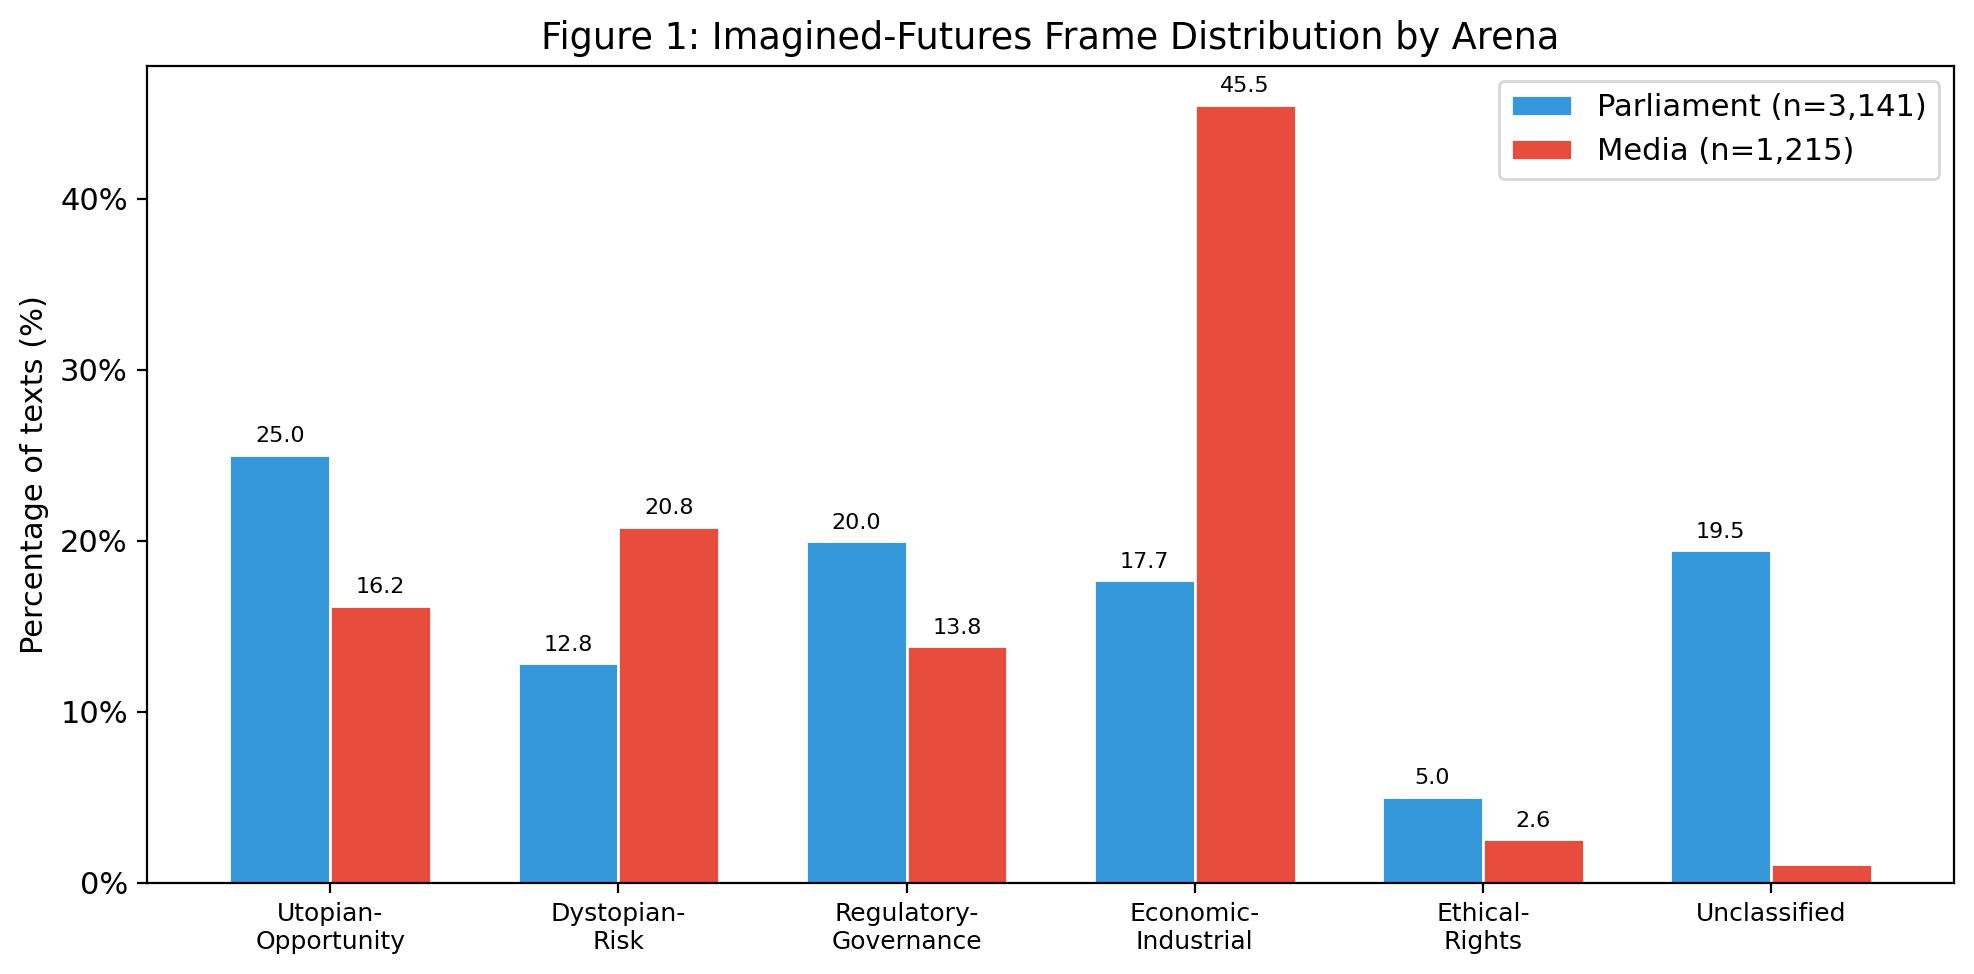
\includegraphics[width=\textwidth]{figures/fig1_frames_by_arena.png}
\caption{Imagined-futures frame distribution by arena. Parliament shows pluralistic framing; media is dominated by the economic-industrial frame.}
\label{fig:frames-arena}
\end{figure}

This arena-level divergence has implications for democratic deliberation. If the public primarily encounters AI discourse through media, the imagined futures available to citizens are narrower and more commercially oriented than those debated in Parliament. The regulatory-governance frame, which in Parliament accounts for one in five utterances and encompasses critical questions about oversight, standards, and institutional design, drops to 13.8\% of media coverage. The ethical-rights frame nearly vanishes. \textcite{friedrich2024}'s warning about the crowding out of alternative futures finds empirical support here: the media arena systematically narrows the diversity of imagined AI futures available to public audiences.

\section{Sentiment Patterns}

The triangulated sentiment analysis reveals substantial differences between arenas. Table~\ref{tab:sentiment-arena} and Figure~\ref{fig:sentiment-dist} summarise the key sentiment metrics.

\begin{table}[htbp]
\centering
\caption{Sentiment analysis by arena (combined VADER + DistilBERT score)}
\label{tab:sentiment-arena}
\begin{tabular}{lrrrr}
\hline
\textbf{Arena} & \textbf{Mean} & \textbf{Positive (\%)} & \textbf{Negative (\%)} & \textbf{Neutral (\%)} \\
\hline
Parliament & $+0.429$ & 63.3 & 25.5 & 11.2 \\
Media & $-0.100$ & 4.8 & 36.5 & 58.8 \\
\hline
\end{tabular}
\end{table}

\begin{figure}[htbp]
\centering
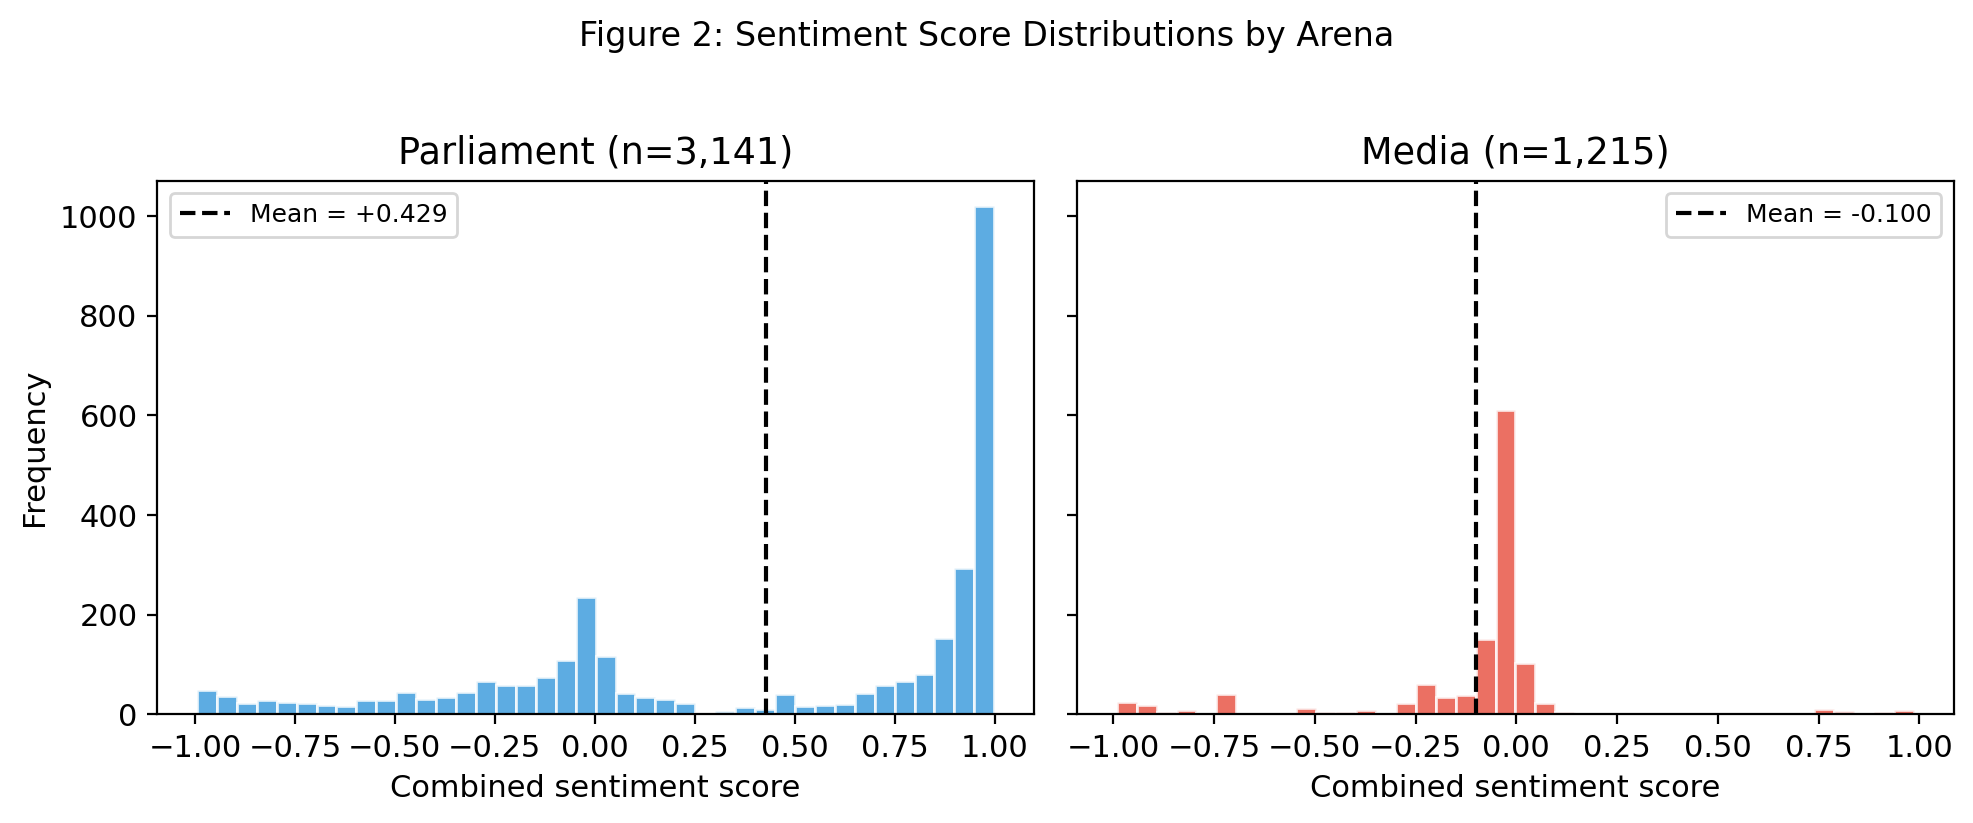
\includegraphics[width=\textwidth]{figures/fig2_sentiment_distributions.png}
\caption{Sentiment score distributions by arena. Parliament clusters positively; media clusters near zero with a negative lean.}
\label{fig:sentiment-dist}
\end{figure}

Parliamentary discourse exhibits a moderately positive average sentiment of $+0.429$, with 63.3\% of utterances classified as positive and 25.5\% as negative. Media statements, by contrast, show a negative average sentiment of $-0.100$, with only 4.8\% classified as positive and 36.5\% as negative, while the majority (58.8\%) fall in the neutral range. The stark sentiment gap between arenas---a difference of over half a point on the combined scale---indicates that media discourse on AI is substantially more cautious and critical than parliamentary discourse. The low proportion of positive media texts suggests that when politicians' AI statements reach public audiences, they tend to be filtered through frames of concern, risk, or measured assessment rather than enthusiasm.

\begin{figure}[htbp]
\centering
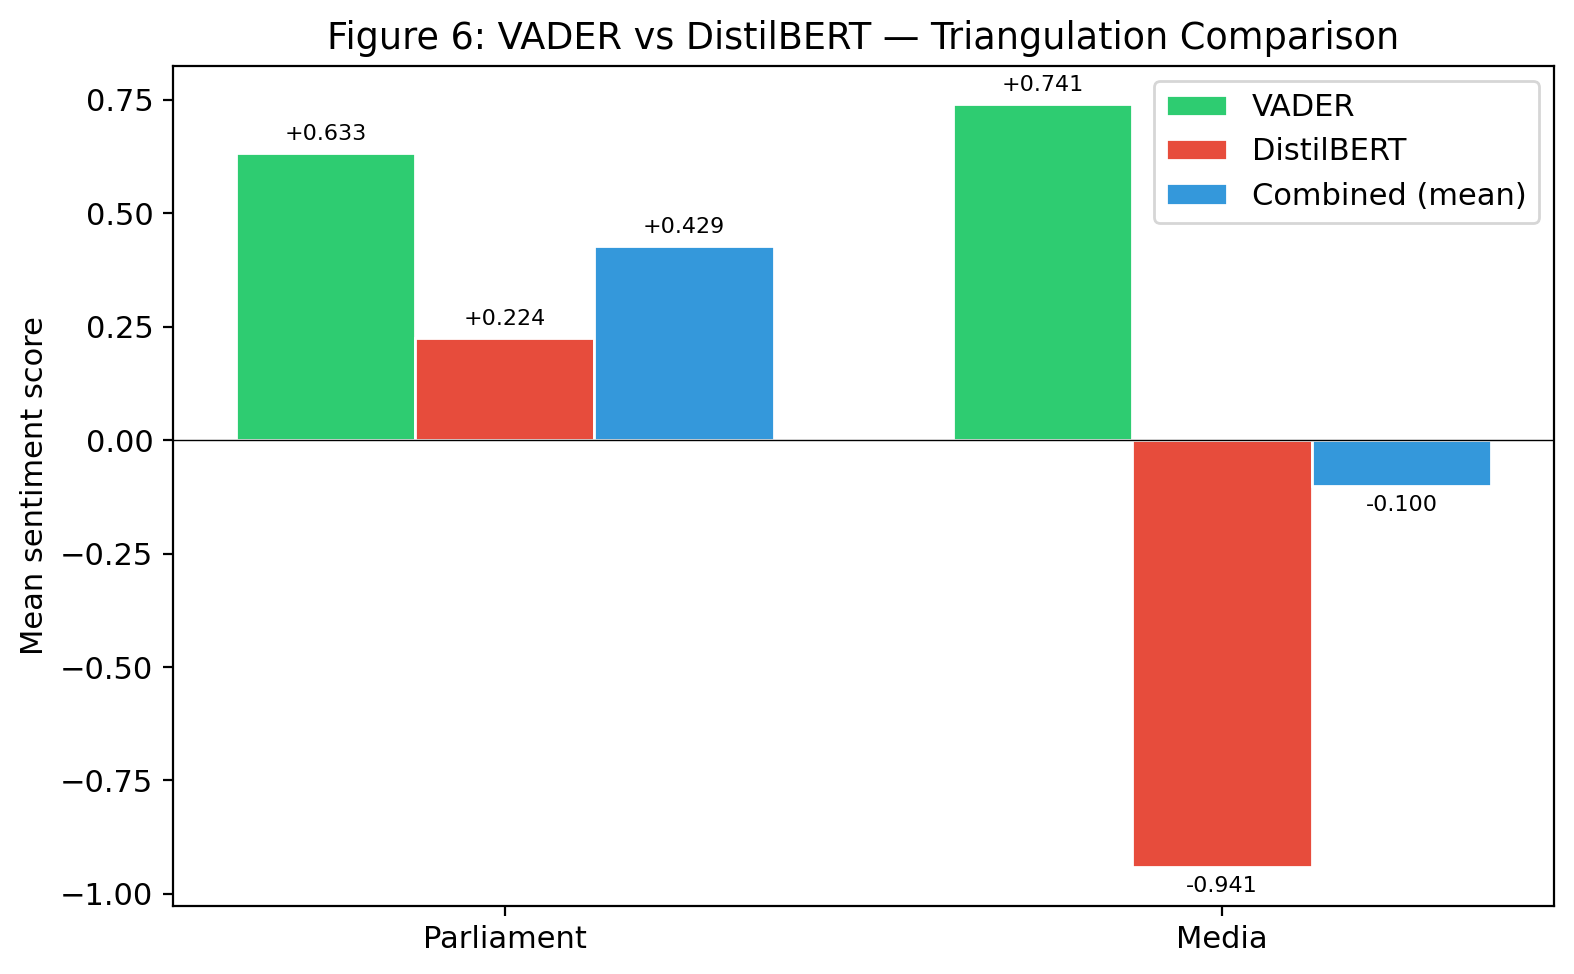
\includegraphics[width=0.85\textwidth]{figures/fig6_vader_vs_distilbert.png}
\caption{VADER vs DistilBERT triangulation. VADER scores both arenas positively; DistilBERT detects strongly negative contextual sentiment in media.}
\label{fig:triangulation}
\end{figure}

The divergence between the two underlying models is itself informative (Figure~\ref{fig:triangulation}). VADER, which relies on lexicon-based valence detection, produced positive mean scores in both arenas (parliament: $+0.633$; media: $+0.741$), reflecting the prevalence of positively valenced words such as ``opportunity'', ``innovation'', and ``growth'' in AI discourse regardless of context. DistilBERT, which captures contextual sentiment at the sentence level, produced a positive score for parliament ($+0.224$) but a strongly negative score for media ($-0.941$). This divergence highlights the value of the triangulation approach: VADER captures surface-level optimistic language that pervades AI discourse, while DistilBERT detects the underlying critical or cautionary framing that contextualises that language---particularly in media texts where positive vocabulary is often embedded in negative or sceptical sentences.

\section{Party-Level Analysis}

The analysis reveals distinct imagined-futures profiles across political groups, reflecting the ideological orientations and institutional positions of each party. Table~\ref{tab:party-sentiment} and Figure~\ref{fig:party-sentiment} present sentiment and frame data for major parties.

\begin{table}[htbp]
\centering
\caption{Sentiment and dominant frames by party}
\label{tab:party-sentiment}
\begin{tabular}{lrrll}
\hline
\textbf{Party} & \textbf{$n$} & \textbf{Mean sent.} & \textbf{Top frame} & \textbf{Parl. / Media} \\
\hline
Conservative & 1,497 & $+0.287$ & Economic-ind. & $+0.509$ / $-0.073$ \\
Labour & 1,203 & $+0.308$ & Economic-ind. & $+0.475$ / $-0.114$ \\
Liberal Dem. & 374 & $+0.042$ & Regulatory-gov. & $+0.130$ / $-0.142$ \\
Crossbench & 274 & $+0.170$ & Economic-ind. & $+0.283$ / $-0.172$ \\
SNP & 65 & $+0.113$ & Economic-ind. & $+0.168$ / $-0.055$ \\
Green & 43 & $-0.008$ & Economic-ind. & $+0.084$ / $-0.114$ \\
\hline
\end{tabular}
\end{table}

\begin{figure}[htbp]
\centering
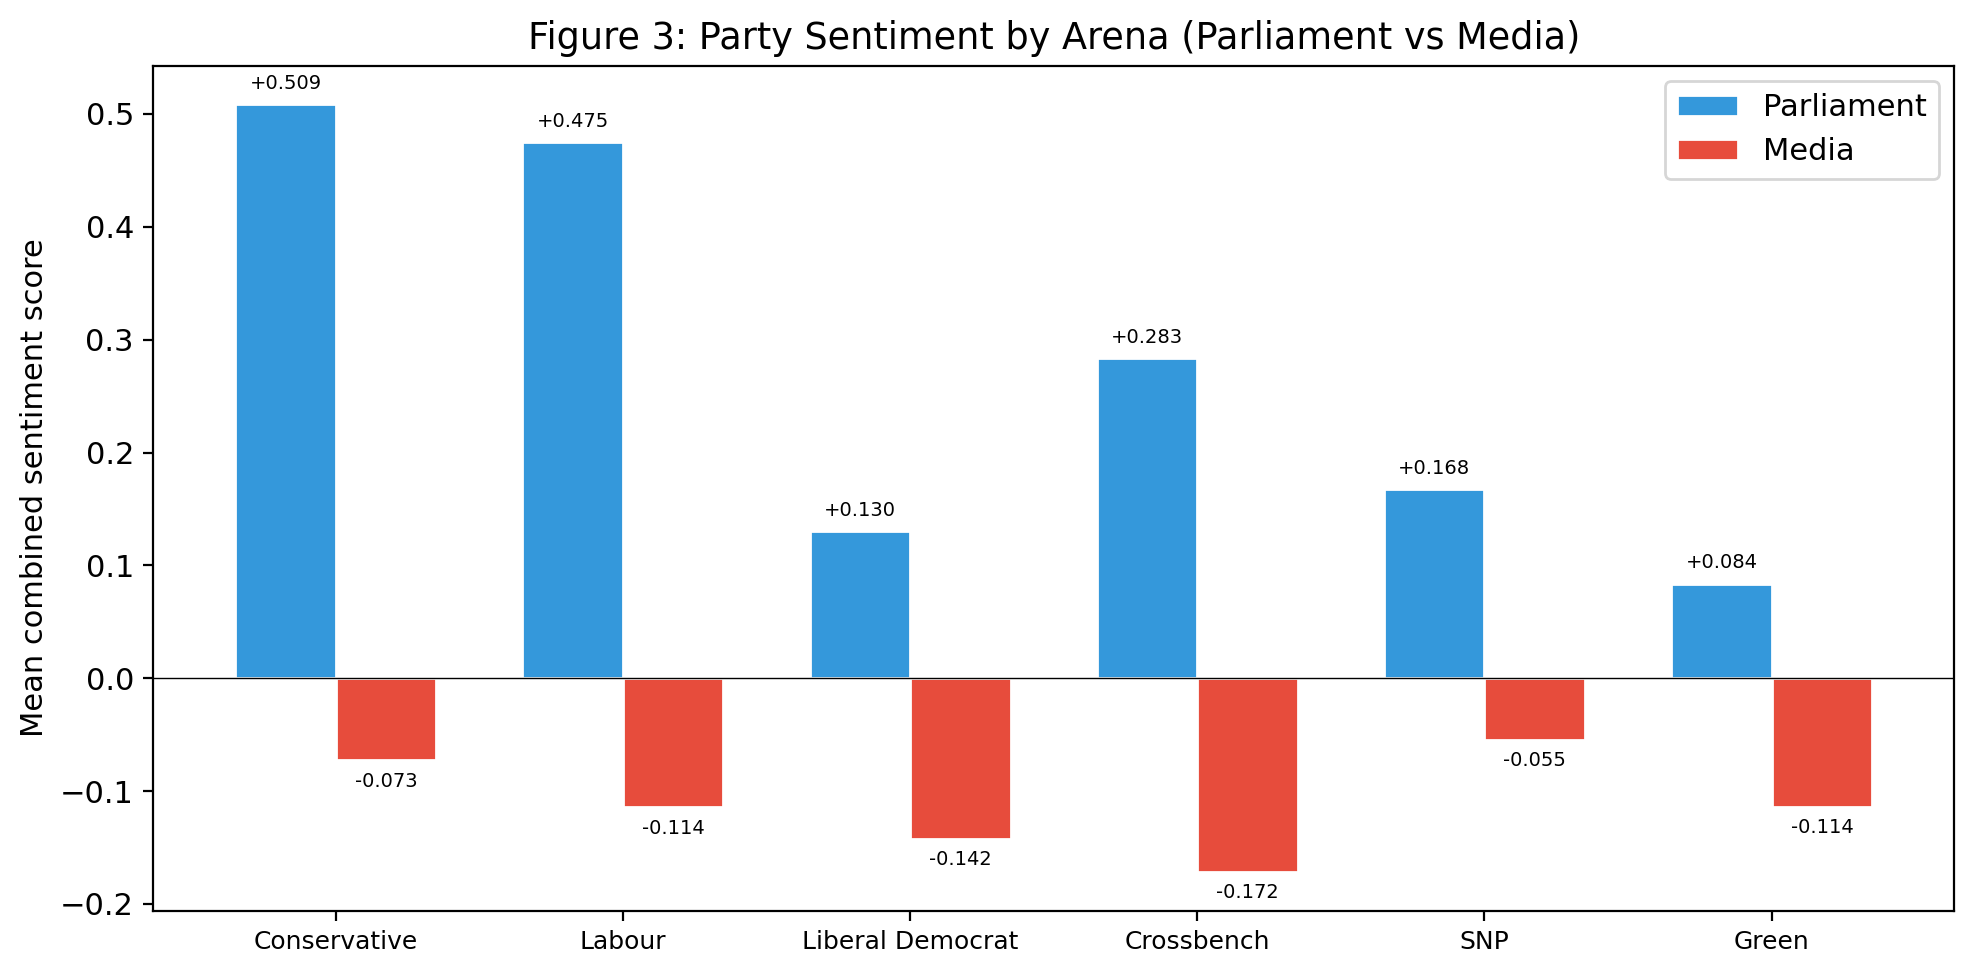
\includegraphics[width=\textwidth]{figures/fig3_party_sentiment_by_arena.png}
\caption{Party sentiment by arena. Every party shifts from positive in Parliament to negative in media.}
\label{fig:party-sentiment}
\end{figure}

\begin{figure}[htbp]
\centering
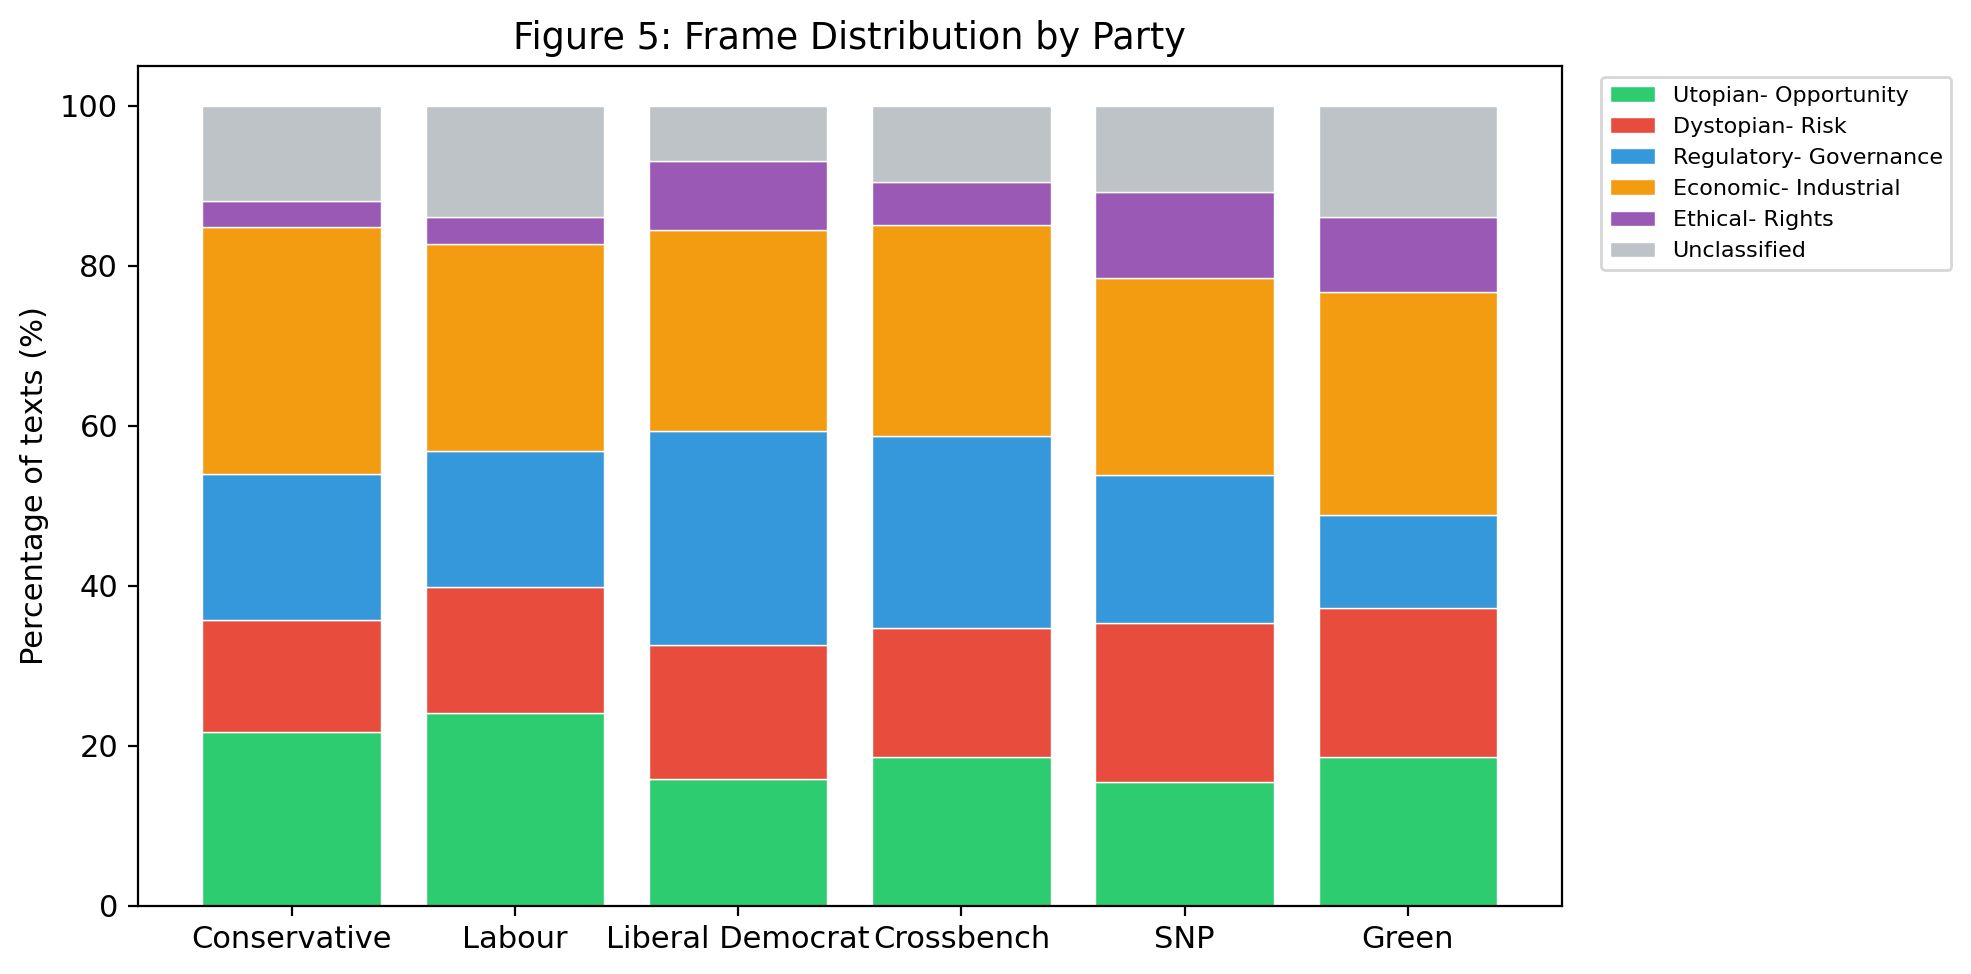
\includegraphics[width=0.85\textwidth]{figures/fig5_frames_by_party.png}
\caption{Frame distribution by party. Economic-industrial and utopian-opportunity dominate across parties, with Liberal Democrats showing a distinctive regulatory-governance emphasis.}
\label{fig:frames-party}
\end{figure}

Labour ($n=1{,}203$), as the governing party from 2024, exhibits the second-highest positive sentiment ($+0.308$) among major parties. In Parliament, Labour is most associated with the utopian-opportunity frame (sentiment $+0.475$), consistent with the Starmer government's AI Opportunities Action Plan and its rhetorical emphasis on AI as a vehicle for public service modernisation and economic growth. Labour's media presence shifts to economic-industrial framing with sentiment dropping to $-0.114$, suggesting a communicative pattern where commercial benefits are emphasised when addressing public audiences but the overall tone becomes more cautious.

The Conservative Party ($n=1{,}497$), which governed until 2024 and initiated the Bletchley Park summit and AI Safety Institute, shows a positive average sentiment of $+0.287$. In Parliament, Conservatives favour the utopian-opportunity frame with the highest arena-specific sentiment of any party ($+0.509$), reflecting both their incumbency optimism and their role in designing the UK's ``pro-innovation'' regulatory architecture. In media, however, Conservatives shift to the economic-industrial frame with sentiment dropping to $-0.073$. This arena shift mirrors Labour's pattern and suggests that the narrowing of AI discourse in media is not a partisan construction but a structural phenomenon affecting both major parties.

The Liberal Democrats ($n=374$) present the most distinctive profile among major parties. Their average sentiment is low ($+0.042$), and they are most strongly associated with the regulatory-governance frame. This reflects the Liberal Democrats' consistent parliamentary emphasis on data protection, civil liberties, and institutional oversight---a position aligned with their broader political identity as advocates for rights and regulatory scrutiny. Their near-zero sentiment score indicates balanced rather than enthusiastic discourse, characterised more by questioning and scrutiny than by advocacy.

The Scottish National Party ($n=65$) shows a mildly positive overall sentiment ($+0.113$). In Parliament, the SNP's top frame is dystopian-risk (sentiment $+0.168$), while in media the dominant frame shifts to economic-industrial with sentiment dropping to $-0.055$. Crossbench peers ($n=274$), often drawn from technical, legal, and academic backgrounds, favour the regulatory-governance frame in Parliament (sentiment $+0.283$), but their media presence ($n=68$) is notably negative ($-0.172$) with an economic-industrial frame. The Green Party ($n=43$) shows near-zero overall sentiment ($-0.008$), with a shift from near-neutral parliamentary discourse to negative media coverage ($-0.114$).

\section{Arena Shifts Within Parties}

A particularly revealing pattern emerges when examining how the same party's discourse shifts between parliamentary and media arenas (Figure~\ref{fig:arena-shift}). Every major party in the dataset exhibits the same structural pattern: positive sentiment and pluralistic framing in Parliament, negative sentiment and economic-industrial dominance in media. This universality is striking and suggests that the arena effect operates independently of partisan ideology.

\begin{figure}[htbp]
\centering
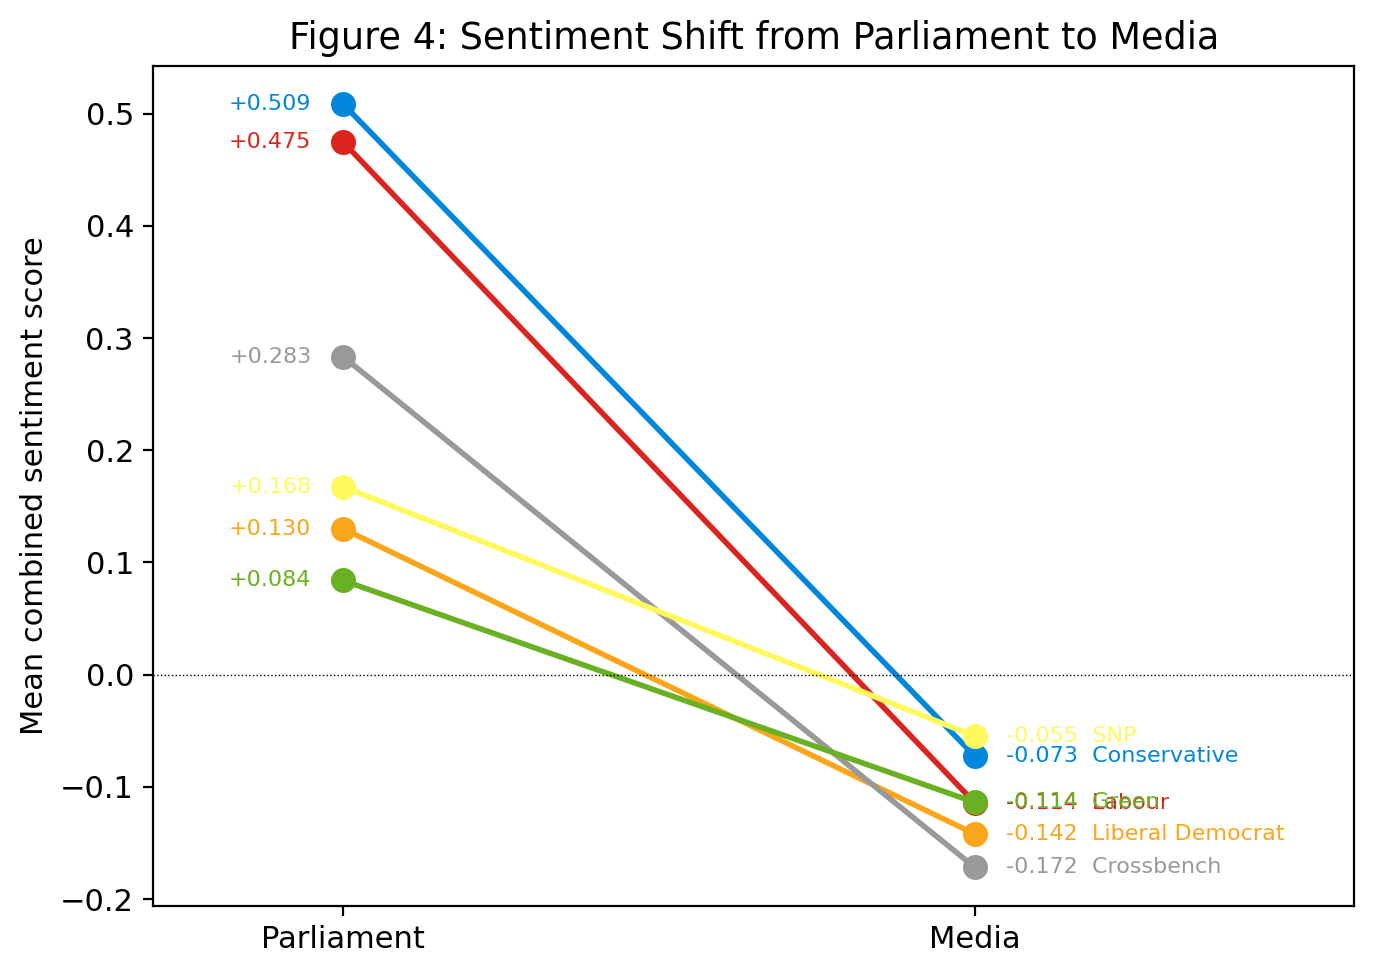
\includegraphics[width=0.8\textwidth]{figures/fig4_arena_shift_slopes.png}
\caption{Sentiment shift from Parliament to media by party. All parties converge into a narrow negative band in media, regardless of their parliamentary starting point.}
\label{fig:arena-shift}
\end{figure}

For Labour, the dominant frame in Parliament is utopian-opportunity (sentiment $+0.475$), reflecting the government's emphasis on AI as a transformative force for public services and national competitiveness. In media, Labour's dominant frame shifts to economic-industrial with sentiment dropping sharply to $-0.114$. This suggests that Labour's media communication de-emphasises the aspirational, public-service-oriented narrative---and that media selection effects may favour more critical or commercially framed statements over optimistic ones.

The Conservative shift follows the same direction but from a higher parliamentary baseline. Parliamentary sentiment of $+0.509$ (the highest of any party in any arena) drops to $-0.073$ in media, a swing of nearly 0.6 points on the combined scale. The dominant frame shifts from utopian-opportunity in Parliament to economic-industrial in media. This pattern suggests that Conservative politicians' most widely reported AI statements tend to be commercially oriented rather than aspirational, and that the media environment transforms even enthusiastic parliamentary advocacy into more measured or critical coverage.

The Liberal Democrats exhibit the smallest absolute swing but the same direction: from $+0.130$ (regulatory-governance frame) in Parliament to $-0.142$ (economic-industrial frame) in media. The consistency of the regulatory-governance frame in Parliament, combined with the shift to economic-industrial in media, suggests that the Liberal Democrats' distinctive focus on oversight and rights is particularly poorly transmitted through media channels.

These within-party arena shifts provide strong evidence for the theoretical claim that futures-making is context-dependent. The same political actors construct meaningfully different imagined futures depending on whether they are operating within the institutional constraints of Parliament or the communicative demands of public media engagement. This is not simply a matter of tone or emphasis: the dominant frame category itself changes between arenas for every major party analysed. The finding has implications for researchers studying political discourse on emerging technologies: analyses that rely exclusively on either parliamentary or media data are likely to capture only a partial and potentially misleading picture of how political actors imagine technological futures.

\chapter{Discussion and Conclusion}

This study set out to investigate how UK political actors imagine the future of artificial intelligence and how these imagined futures vary across political arenas and parties. The findings offer several contributions to the understanding of futures-making in technology policy.

The first and most striking finding is the systematic divergence between parliamentary and media discourse. Parliament sustains a relatively pluralistic ecology of imagined futures, with substantial representation of utopian, regulatory, dystopian, economic, and ethical framings. Media discourse, by contrast, is dominated by economic-industrial narratives that foreground investment, competitiveness, and commercial opportunity. This divergence holds across all parties: every major political group shifts from positive, pluralistic framing in Parliament to negative, economically dominated framing in media. The implication is that the media arena does not merely transmit parliamentary discourse to public audiences but actively reshapes it, narrowing the range of imagined futures that citizens encounter. This finding resonates with \textcite{friedrich2024}'s observation that dominant imagined futures can crowd out alternatives, and suggests that in the UK context, the economic-industrial imagined future of AI enjoys a structural advantage in public communication.

The hypothesis that arena shapes imagined futures receives strong support. The sentiment gap between arenas---$+0.429$ in Parliament versus $-0.100$ in media---is substantial and consistent across parties. Moreover, the triangulation between VADER and DistilBERT revealed that this gap is driven primarily by contextual sentiment (captured by the transformer model) rather than surface vocabulary: politicians use similarly positive AI-related terminology in both settings, but the framing context in media is markedly more critical.

The second finding concerns party-level variation. The analysis confirms that different political groups construct systematically different imagined futures, in ways that align with their broader ideological commitments and institutional positions. Labour's utopian-opportunity orientation, the Conservatives' high-sentiment parliamentary enthusiasm, the Liberal Democrats' rights-oriented scrutiny, and the Crossbench peers' regulatory focus each reflect distinct political projects and represent different answers to the question of what AI will mean for British society. This pluralism at the party level is a positive finding for democratic deliberation: it indicates that the political system generates a diversity of imagined futures, even if media representation compresses this diversity.

The dual-method sentiment analysis adds analytical value beyond what either model alone could provide. VADER's consistently positive scores across arenas demonstrate that AI discourse is saturated with optimistic vocabulary regardless of the speaker's actual evaluative stance. DistilBERT's ability to detect contextual criticism beneath this positive vocabulary---particularly its strongly negative media score of $-0.941$---reveals a layer of meaning that lexicon-based approaches alone would miss. The triangulation approach thus captures both the surface rhetoric and the underlying evaluative orientation of political AI discourse.

Several limitations should be acknowledged. The keyword-based frame classification, while transparent and reproducible, lacks the contextual sensitivity of manual coding or supervised machine learning. The ParlaMint corpus extends only to mid-2022, meaning that the most recent parliamentary data comes exclusively from Hansard, introducing potential variation in text processing. The media dataset, while substantially larger than in comparable studies ($n=1{,}215$ across 127 politicians), may still reflect selection biases in web search retrieval. Additionally, the inclusion of House of Lords members in both datasets---while justified by their substantive role in AI scrutiny---means that the parliamentary dataset is not limited to elected officials. Some LDA topics contain artefacts from web-scraped media content (navigation text, subscription prompts), which, while filtered from the frame classification through custom stop words, affect the interpretability of certain topic labels.

Despite these limitations, the study demonstrates the analytical value of applying the imagined-futures framework to computational text analysis of political discourse. By combining topic modelling, dual-method sentiment analysis, and frame classification with a theoretically grounded comparative design, it has been possible to identify systematic patterns in how UK politicians construct narratives about AI's future---patterns that would be difficult to detect through close reading of individual debates or media reports.

Future research could extend this approach in several directions. A longitudinal analysis tracking the evolution of imagined futures across key policy moments---the Bletchley Park summit, the 2024 election, the Regulating AI for Growth Bill---would capture the dynamic character of futures-making. Supervised classification models trained on manually labelled data could improve the precision of frame detection. Cross-national comparison with EU member states, where the regulatory imagined future has been codified in the AI Act, would illuminate how institutional context shapes the range of futures that political actors construct.

In conclusion, UK political discourse on artificial intelligence is fundamentally oriented toward the future, and the futures that politicians imagine are shaped by both partisan ideology and communicative context. Parliament sustains a diverse ecology of imagined futures. Media compresses this diversity into predominantly economic-industrial narratives while shifting the overall evaluative tone from positive to negative. Understanding these dynamics is essential for anyone seeking to assess how democratic societies are navigating the deep uncertainties of artificial intelligence.
